% !TEX program = xelatex

\documentclass{beamer}
\usetheme{default}

\usepackage{ctex}

\title{Blockchain at the Edge: Performance of Resource-Constrained IoT Networks}
\author{张展鹏}
\begin{document}
\begin{frame}[plain]
    \maketitle
\end{frame}

\begin{frame}{物联网安全现状}
	器件差异性、局限性和传统安全方法面临的困难
	\begin{itemize}
		\item 物联网设备是海量的,设备间差异非常大,大部分是边缘设备;
		\item 边缘设备任务简单,专注于完成特定的简单任务和低功耗网络连接,几乎无多余的资源承载额外的安全机制;
		\item 物联网设备自身存在系统性和习惯性安全缺陷,例如弱密码、硬编码(固定)固码、缺乏安全访问的接口、不安全的数据访问和传输机制等;
		\item 物联网设备海量且空间位置不确定,管理员很难查找被感染或恶意设备;
		\item 当前主流的物联网安全方案依赖于集中式物联网网关,它会管理它负责的范围内物联网设备,目前物联网边缘快速拓展,集中式网关在长期难以适应这样的发展趋势。
	\end{itemize}
\end{frame}

\begin{frame}{物联网的“两域”和“六层”}
	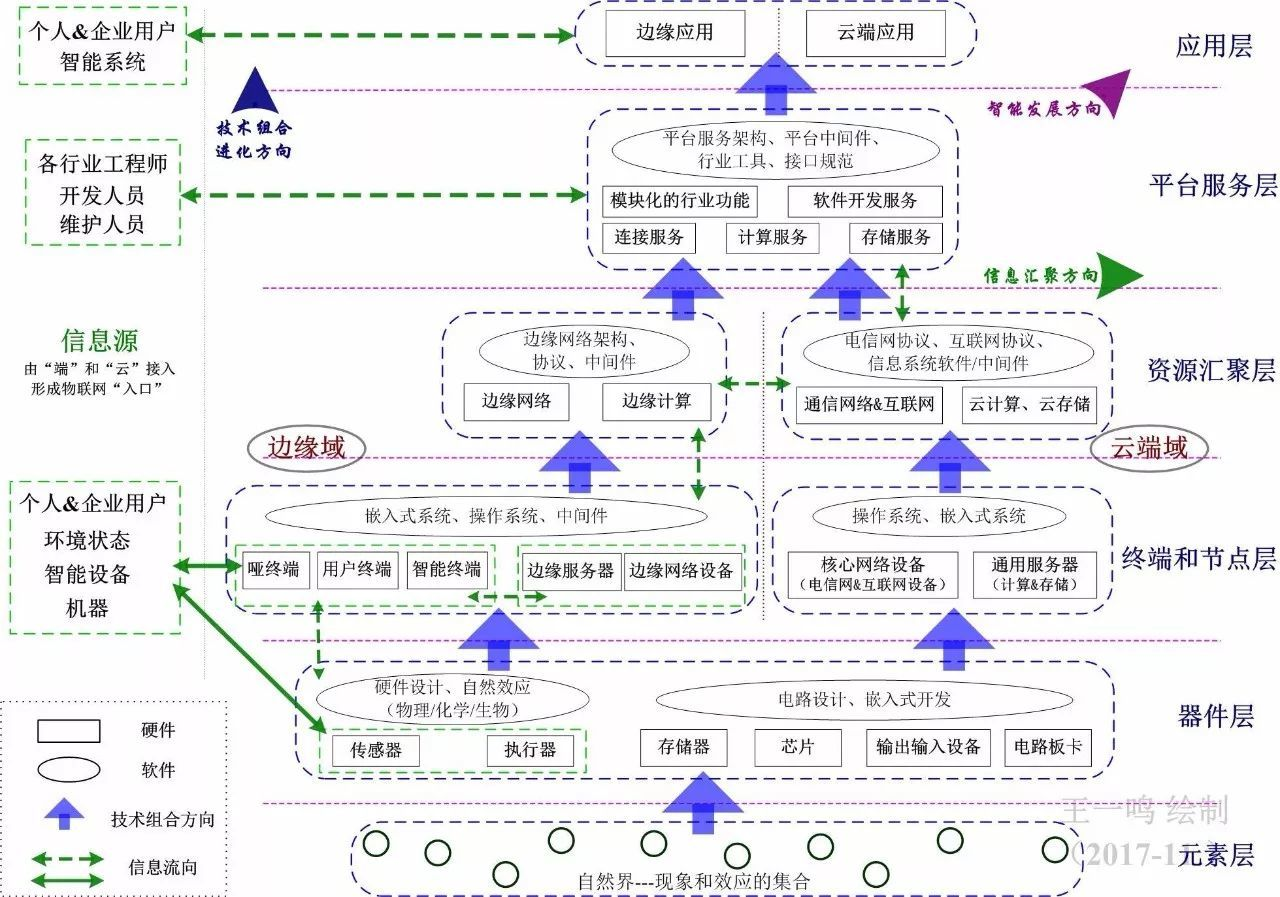
\includegraphics[width=\linewidth]{Assets/v2-7855b4b4d5101e18dc398cb0ca92d141_1440w}
\end{frame}

\begin{frame}{总体思路:从集中式到分布式}
	集中式网关的缺陷和分布式解决方案
	\begin{itemize}
		\item 集中式网关 v.s. 分布式网关
		\begin{itemize}
			\item 集中式网关位于资源汇聚层,由指定设备完成协议转换和流量转发,适合简单的一对多;集中式网关决定了它管理的全体设备的MAC地址,这意味着集中式网关的可拓展性差;
			\item 分布式网关位于终端和节点层,数量多、适合自动化部署、配置灵活、扩展性良好,分布式网关的流量转发路径最优。
		\end{itemize}
		\item 集中式网关不适合物联网,它无法阻止未经授权直接访问物联网边缘的行为,集中式网关依赖远程托管的安全机制,必然依赖云端管理者和集中式网关。
		\item 分布式系统的拓展性决定了它更适合作为物联网安全解决方案。区块链是典型的安全的分布式系统,链上数据不可篡改——区块链+物联网。
	\end{itemize}
\end{frame}

\begin{frame}{区块链应用在物联网的挑战}
	运算能力和网络状况
	\begin{itemize}
		\item 物联网设备越多,链上节点越多,每个链上节点,即物联网设备的运算和存储压力越大,物联网边缘设备不是为执行大量运算设计的,也不全有存储设备;
		\item 物联网设备的网络连接是受限的,链上节点必须同步数据,大多数物联网边缘设备无内部时钟,这类非实时性设备很难进行主动同步。
	\end{itemize}
\end{frame}

\begin{frame}{论文的模拟和解决方法}
	论文工作在4节点以太坊区块链展开,针对在运算能力和网络状况遇到的问题分别进行了模拟和解决。
	\begin{itemize}
		\item 为了模拟设备多样性和网络多样性,4个节点包括了以太网和我Wi-Fi连接的工作站和树莓派;
		\item 作者提出了一种可以应用在区块链中的中心化时间同步机制,通过传统的授时方案实现无内部时钟设备的时间设置和同步,这样的时间字符串是密文传输的。
	\end{itemize}
\end{frame}

\begin{frame}{基于区块链的物联网授时服务架构}
	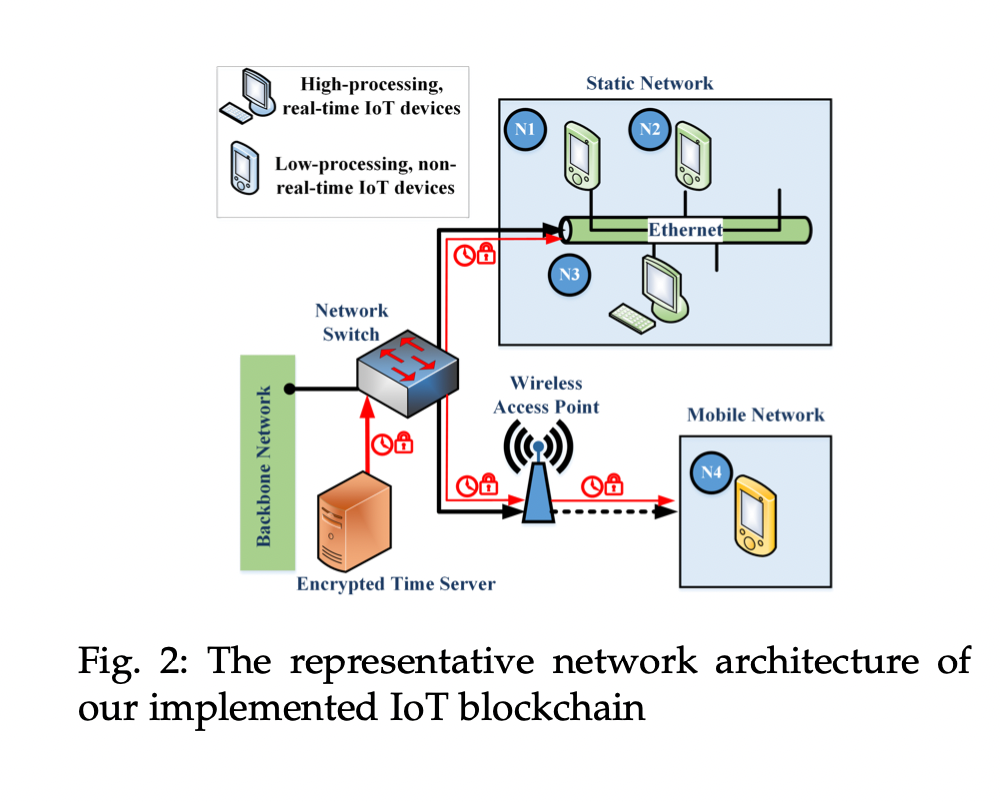
\includegraphics[width=\linewidth]{Assets/图2}
\end{frame}

\begin{frame}{节点资源列表}
	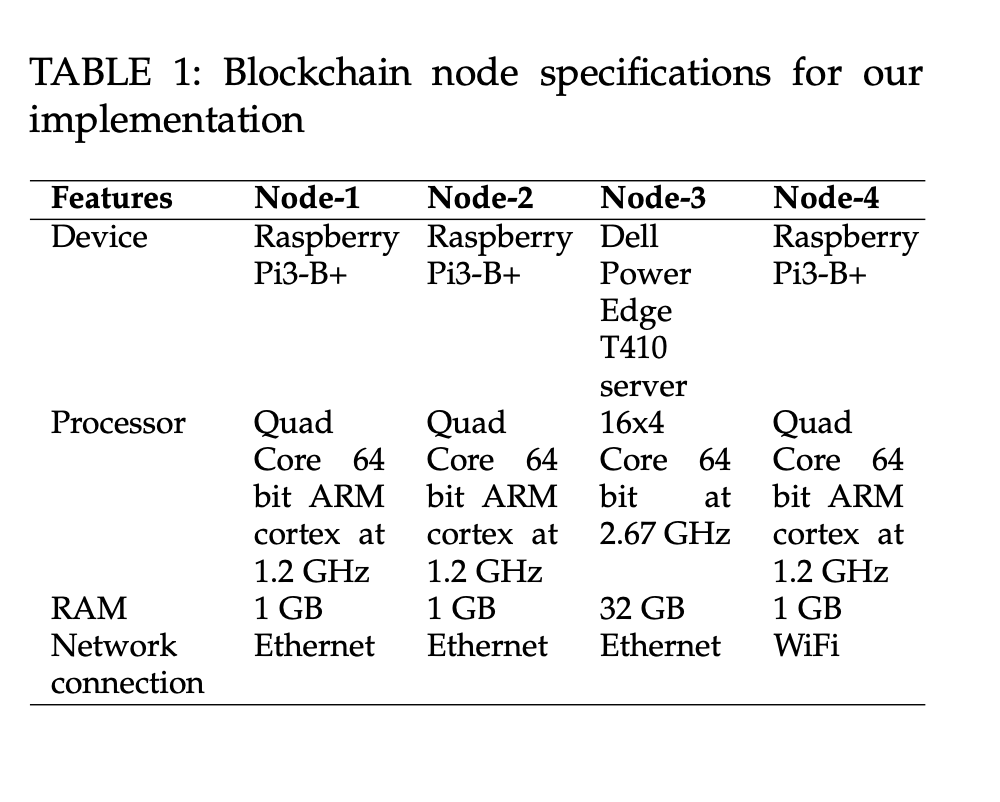
\includegraphics[width=\linewidth]{Assets/表1}
\end{frame}

\begin{frame}{以太坊私链设置}
	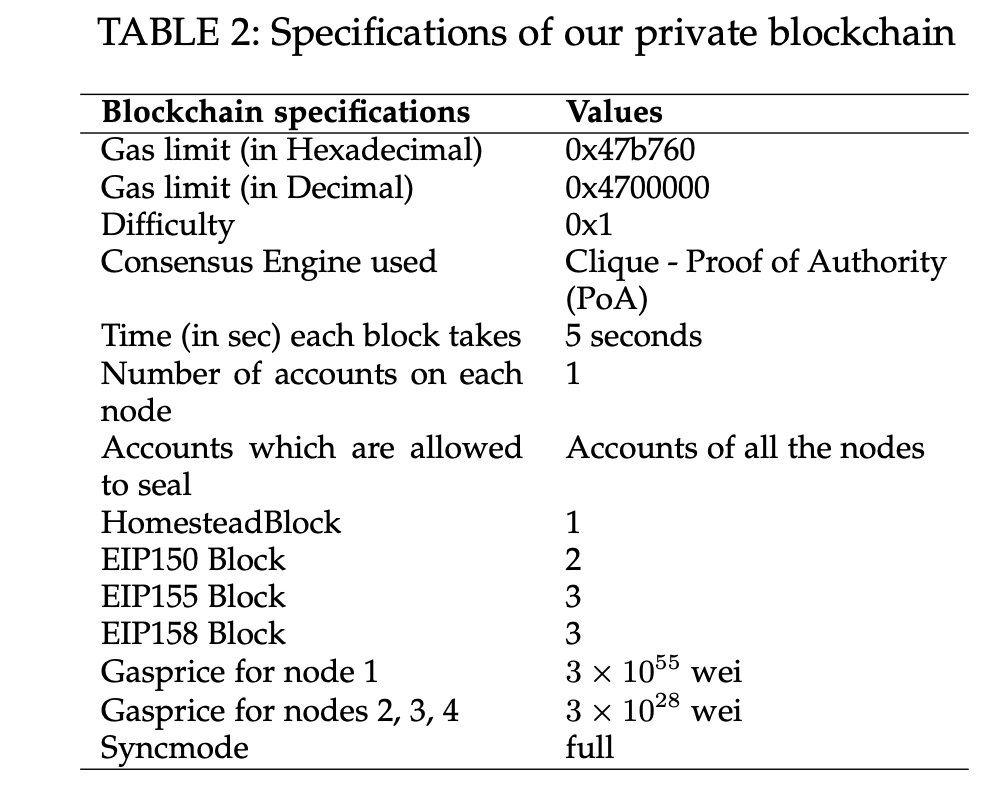
\includegraphics[width=\linewidth]{Assets/表2}
\end{frame}

\begin{frame}{节点的链上动作——交易和挖矿}
	论文要求物联网边缘设备节点同样具备发起交易和挖矿的功能。
	\begin{itemize}
		\item 通过极低的难度(difficulty),在大部分节点计算能力匮乏的情况下控制了5s的出块时间;
		\item 使用PoA(权威共识),由权威节点验证交易并提供同步服务,记账仍然是分布式的,它的性能非常高。
		PoA在私链广泛,它是PoS(权益证明)的变体,参与交易验证的抵押物从数字资产变成了身份。它的性能是三种共识机制中最高的,验证节点的权威身份无法挑战。
	\end{itemize}
\end{frame}

\begin{frame}{为什么PoA共识机制下也需要全体节点参与挖矿?}
	\begin{itemize}
		\item 实验链使用了PoA机制,实验中,节点仍然需要挖矿。既然物联网边缘设备的计算资源匮乏,验证节点(Node-3,服务器)可以成为唯一矿工且拥有完全记账权,为什么每个节点还是需要挖矿?\\
		Irrespective of a node’s processing capabilities, the nodes are self-sufficient to carry out \underline{mining} operations on their own ... This drop in connection results in a significant increase in mining times at the affected nodes.
		\item 节点挖矿难度很低,不需要奖励。
	\end{itemize}
\end{frame}

\begin{frame}{节点行为}
	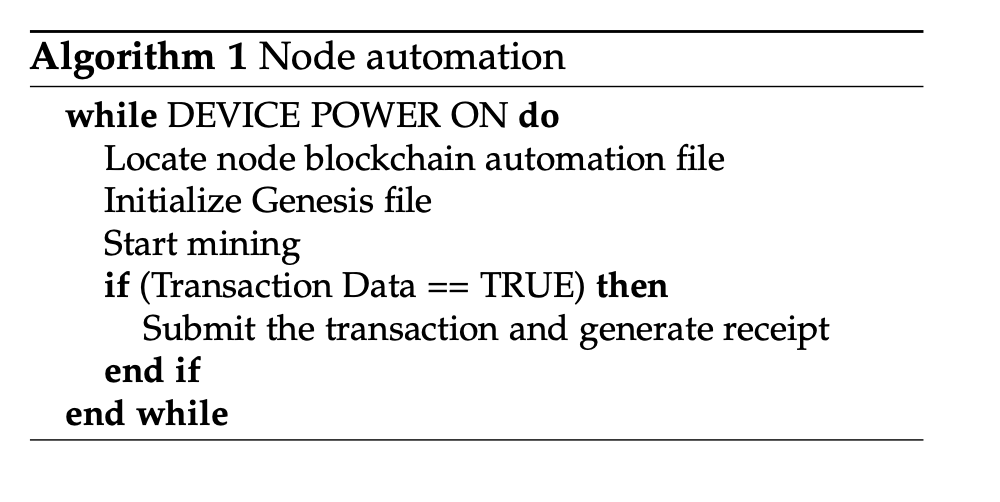
\includegraphics[width=\linewidth]{Assets/算法1}
	挖矿和交易是写死在节点中的。挖矿的主要目的是根据出块时间做节点网络健康状态监控;交易是为了模拟现实世界中物联网终端传输数据的功能。\textbf{写死的交易体意味着物联网边缘设备发送和接收的数据长度是固定的。}
\end{frame}

\begin{frame}{时间同步机制——节点唯一标识}
	论文在这里使用了身份基加密,实际上给每个物联网节点分发了一个密钥,即\texttt{ENODE}。\\
	IoT blockchain nodes have unique “ENODE” values and connect using these values. The “ENODE” value consists of a public key, an IPv4 address, and a port number.\\
	\texttt{ENODE} = ENODE(\texttt{pubKey}, \texttt{IP}, \texttt{port})
\end{frame}

\begin{frame}{时间同步机制——中心化思想}
	物联网边缘设备一般缺少实时时钟(Real-Time Clock),它们的内部时钟会在启动是重置,这要求物联网边缘设备上链和启动时收到时间广播。\\
	广播虽然是无连接的,但是它有明确的目标,需要确保对应设备收到了完整的广播内容且正常解密。
	\begin{itemize}
		\item 授时服务器维护\texttt{IP}和\texttt{ENODE},定期通过广播更新物联网边缘设备的内部\texttt{IP};
		\item 篡改密钥涉及篡改\texttt{IP},两者是一一映射的,这样的行为容易被捕捉。
	\end{itemize}
\end{frame}

\begin{frame}{时间同步机制——算法 (1)}
	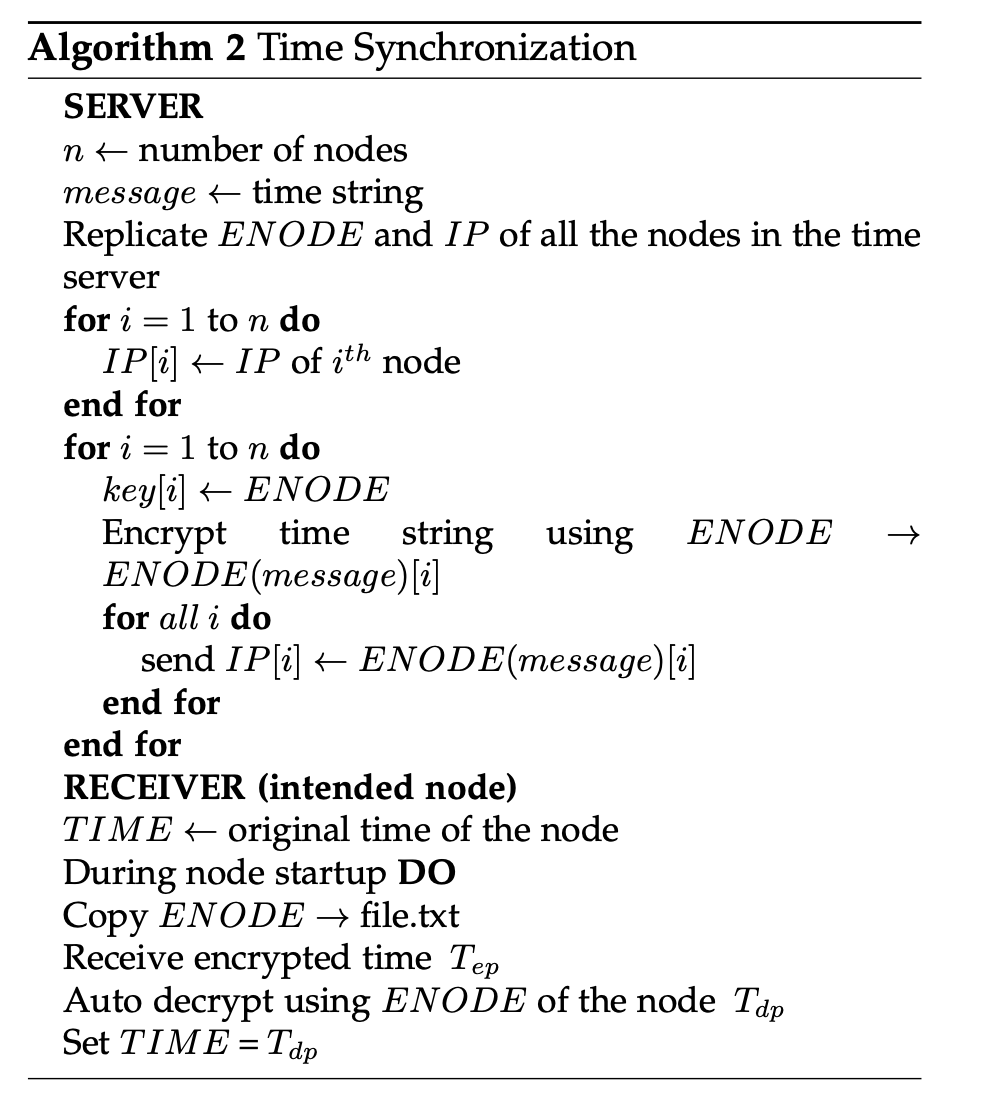
\includegraphics[width=0.618\linewidth]{Assets/算法2}\\
	通过\texttt{IP}建立连接;分发密钥,通过连接正确性确保不被篡改;广播时间密文
\end{frame}

\begin{frame}{时间同步机制——算法 (2)}
	\begin{itemize}
		\item 算法是暴力的,未做时间复杂度层面的优化。授时服务器发送消息是平方时间复杂度,设备接收消息是线性时间复杂度;
		\item 为每一个设备定制密钥和时间密文的方式很难适应物联网的快速增长;
		\item 我们可以维持时间密文不变,预先定义解密组策略(例如基于属性密码设计每个节点的安全策略),这样可以把时间字符串广播的收发双方都优化成常数时间复杂度。
	\end{itemize}
\end{frame}

\begin{frame}{实验数据 (1)——计算资源和网络状态监控}
	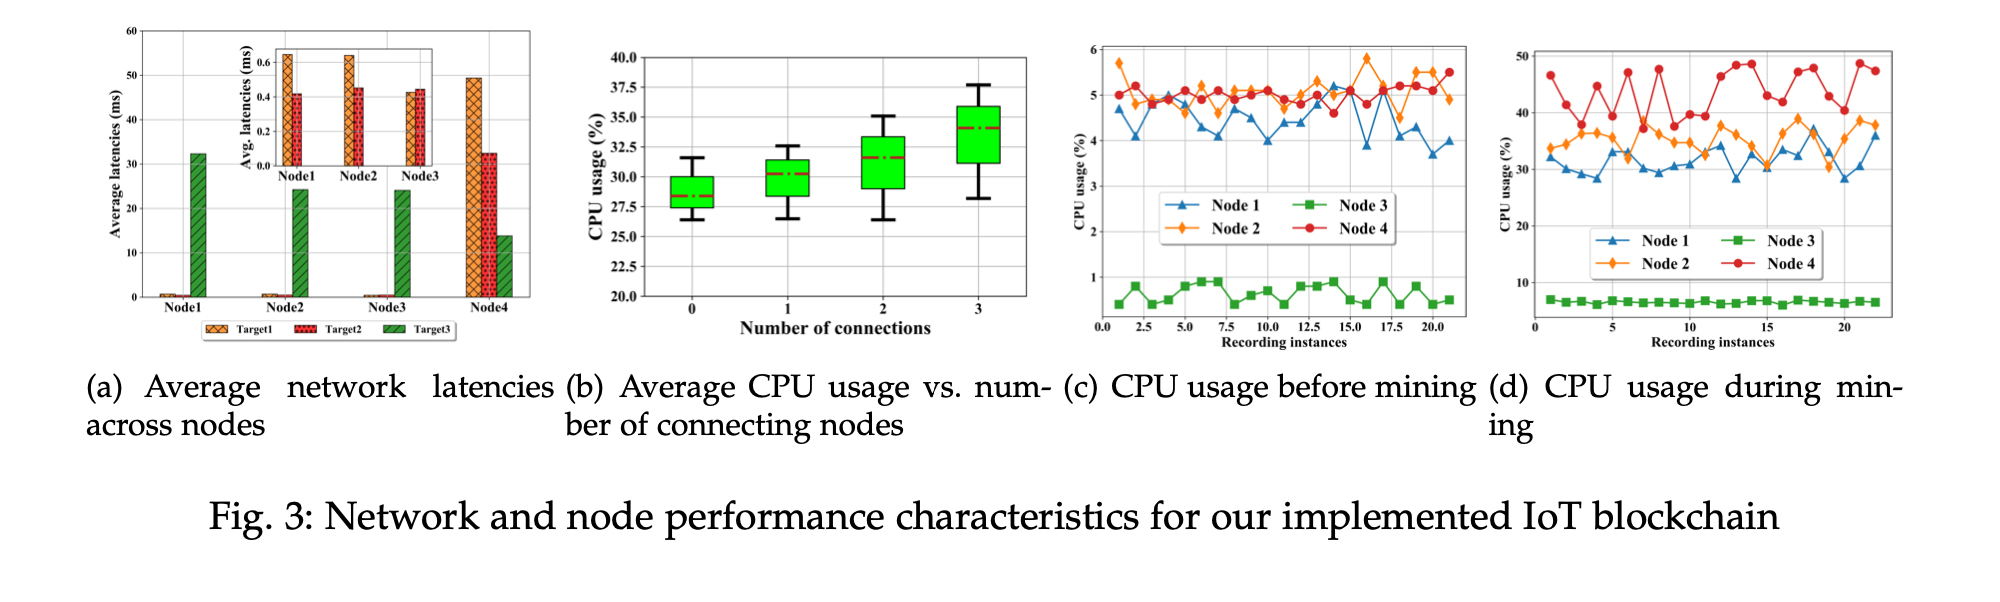
\includegraphics[width=\linewidth]{Assets/图3}
\end{frame}

\begin{frame}{实验数据 (2)——对称/非对称,是否对链上数据加密}
	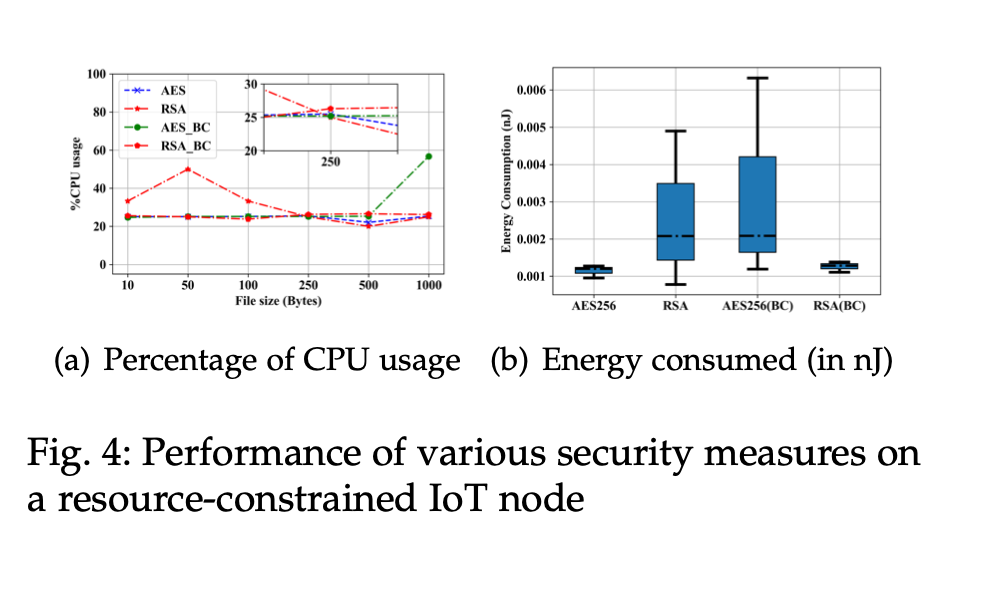
\includegraphics[width=\linewidth]{Assets/图4}
\end{frame}

\begin{frame}{实验数据 (3)——交易数据长度影响性能}
	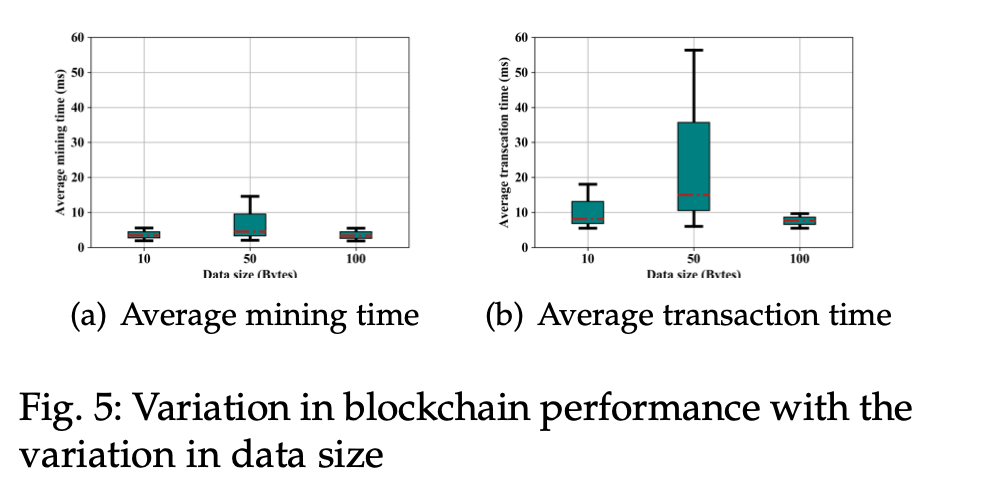
\includegraphics[width=\linewidth]{Assets/图5}
\end{frame}

\begin{frame}{实验数据 (4)——交易金额影响性能}
	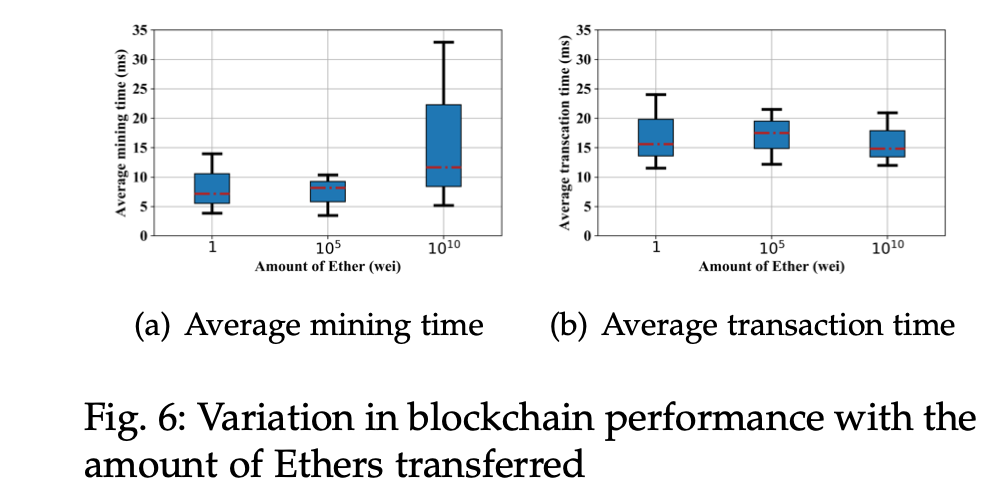
\includegraphics[width=\linewidth]{Assets/图6}
\end{frame}

\begin{frame}{实验数据 (5)——计算资源和网络状态影响性能}
	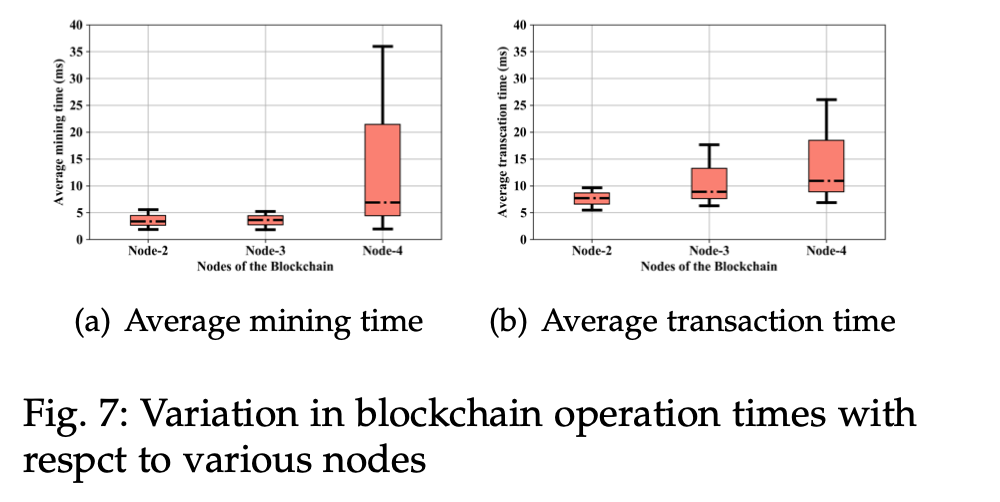
\includegraphics[width=\linewidth]{Assets/图7}
\end{frame}

\begin{frame}{实验数据 (6)——网络延迟监控}
	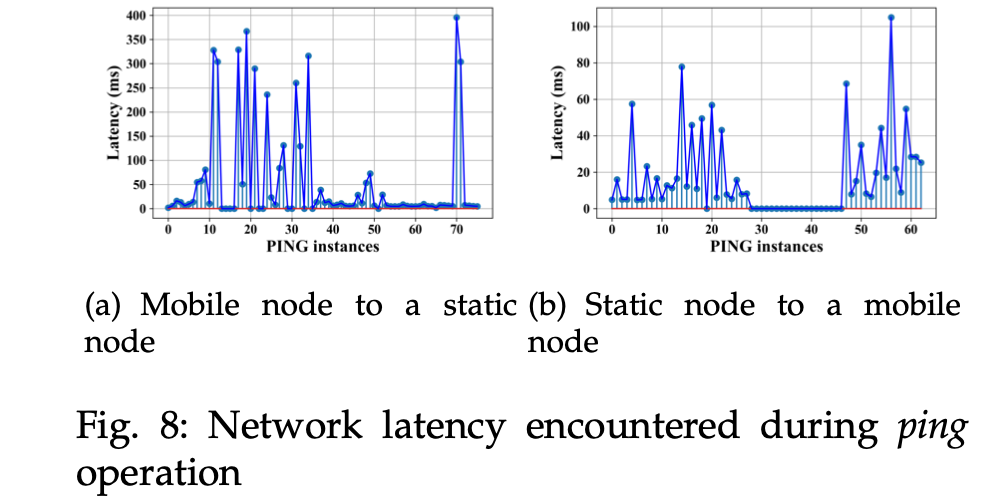
\includegraphics[width=\linewidth]{Assets/图8}
\end{frame}

\begin{frame}{本文特色}
	\begin{itemize}
		\item 实验系统搭建合理,我们在设计区块链+物联网的实验时,一般选用3—4台设备;
		\item 运用PoA,减轻了物联网边缘设备的负载,通过节点挖矿时间了解网络连接状态;
		\item 授时中心的设计思路很简洁,分布式授时远比集中式授时复杂,且面临针对分布式同步机制的攻击;
		\item 在设计基于区块链的物联网解决方案时,Wi-Fi连接的中断问题是一个系统性挑战,它会导致非常显著的性能损失。
	\end{itemize}
\end{frame}

\begin{frame}{本文缺陷}
	\begin{itemize}
		\item 缺少算法复杂度分析,缺少图表分析(描述文字太多);
		\item 授时中心有很大的改进空间,作为原型是足够的,安全组策略在面临海量设备应用问题时是必然需求,可以结合属性密码设计;
		\item 交易灵活性不足,交易是以固定的频率发出的,可以设计大量随机交易进一步测试系统稳定性,目前除了Wi-Fi连接中断,论文未提到其他性能瓶颈。
	\end{itemize}
\end{frame}
\end{document}